% This must be in the first 5 lines to tell arXiv to use pdfLaTeX, which is strongly recommended.
\pdfoutput=1
% In particular, the hyperref package requires pdfLaTeX in order to break URLs across lines.

\documentclass[11pt]{article}

% Remove the "review" option to generate the final version.
\usepackage[]{EACL2023}

% Standard package includes
\usepackage{times}
\usepackage{latexsym}

% For proper rendering and hyphenation of words containing Latin characters (including in bib files)
\usepackage[T1]{fontenc}
% For Vietnamese characters
% \usepackage[T5]{fontenc}
% See https://www.latex-project.org/help/documentation/encguide.pdf for other character sets

% This assumes your files are encoded as UTF8
\usepackage[utf8]{inputenc}
\usepackage{graphicx}
\usepackage{graphicx,xcolor}
\usepackage{multirow}
\usepackage{caption}
\usepackage{subcaption}
\usepackage{amsfonts}
\usepackage{amsmath}
 \usepackage{mathtools}  
\usepackage{subcaption}
\usepackage{xcolor, colortbl}
\usepackage{booktabs}
\usepackage{algorithm}
\usepackage{algorithmic}
\usepackage[utf8]{inputenc}
\usepackage{epsfig}
\usepackage{graphicx}
\usepackage{amssymb}
\usepackage{epsfig}
\usepackage{amsmath}
\usepackage{multirow}

% This is not strictly necessary, and may be commented out.
% However, it will improve the layout of the manuscript,
% and will typically save some space.
\usepackage{microtype}

% This is also not strictly necessary, and may be commented out.
% However, it will improve the aesthetics of text in
% the typewriter font.
\usepackage{inconsolata}


% If the title and author information does not fit in the area allocated, uncomment the following
%
%\setlength\titlebox{<dim>}
%
% and set <dim> to something 5cm or larger.

\title{\textit{READ}: Reinforcement-based Adversarial Learning for Text Classification with Limited Labeled Data}

% Author information can be set in various styles:
% For several authors from the same institution:
% \author{Author 1 \and ... \and Author n \\
%         Address line \\ ... \\ Address line}
% if the names do not fit well on one line use
%         Author 1 \\ {\bf Author 2} \\ ... \\ {\bf Author n} \\
% For authors from different institutions:
% \author{Author 1 \\ Address line \\  ... \\ Address line
%         \And  ... \And
%         Author n \\ Address line \\ ... \\ Address line}
% To start a seperate ``row'' of authors use \AND, as in
% \author{Author 1 \\ Address line \\  ... \\ Address line
%         \AND
%         Author 2 \\ Address line \\ ... \\ Address line \And
%         Author 3 \\ Address line \\ ... \\ Address line}

\author{ Rohit Sharma \quad Shanu Kumar \quad Avinash Kumar\\
Microsoft Corporation, India \\
{\tt \small rohit.sharma@alumni.iitgn.ac.in} {\tt \small \{shankum,avkum\}@microsoft.com} }


\begin{document}
\maketitle
\begin{abstract}
Pre-trained transformer models such as BERT have shown massive gains across many text classification tasks. However, these models usually need enormous labeled data to achieve impressive performances. Obtaining labeled data is often expensive and time-consuming, whereas collecting unlabeled data using some heuristics is relatively much cheaper for any task. Therefore, this paper proposes a method that encapsulates reinforcement learning-based text generation and semi-supervised adversarial learning approaches in a novel way to improve the model's performance. Our method \textit{READ} (\textbf{RE}inforcement-based \textbf{AD}versarial learning) utilizes an unlabeled dataset to generate diverse synthetic text through reinforcement learning, improving the model's generalization capability using adversarial learning. Our experimental results show that \textit{READ} outperforms the existing state-of-art methods on multiple datasets. 

% Language models (LM) such as BERT show high performance on the text classification task. However, language models usually need thousands of labeled data to achieve such high performance. Obtaining a large amount of labeled data is often difficult due to time paucity, operational challenges, and cost considerations. but in contrast, having unlabelled examples characterizing the target task can be collected. In this paper, we propose a novel RL-LM model for text classification, which uses an unlabeled dataset to generate diverse synthetic text in a generative adversarial setting through reinforcement learning. In RL-LM, the weights of the Language Model (BERT, RoBERTa etc.) get fine-tuned using a small set of labeled text along with a synthetic text generation process. RL-LM learns the data distribution of unlabeled datasets during the synthetic text generation process, which helps LM to become highly generalized compared to existing methods. Experimental results show that RL-LM achieves better multi-class classification accuracy in a small labeled dataset setting and outperforms existing state-of-the-art models on multiple real-world datasets.
\end{abstract}

\section{Introduction}
\label{submission}

The introduction of pre-trained transformer-based large-scale models such as BERT \cite{devlin-etal-2019-bert}, GPT-2 \cite{radford2019language}, and RoBERTa \cite{liu2019roberta} has led to impressive results on many Natural Language Processing (NLP) tasks. However, even with a pretraining these models require a large number of labelled data for fine-tuning on a downstream task \cite{yogatama2019learning, croce2020gan}. Few works \cite{mukherjee2020uncertainty, croce2020gan} have shown significant drop in performance while fine-tuning BERT using only limited examples.

Obtaining labelled data can be expensive and time-consuming process \cite{dandapat-etal-2009-complex, sabou2012crowdsourcing, fort2016collaborative}, nevertheless collecting unlabeled data for any downstream task is relatively much cheaper. Semi-supervised learning \cite{kipfsemi, zhu2005semi} has been shown to be one of the promising paradigms to generalize even with few labelled data, by utilizing large amounts of unlabeled data. Recently, \citet{miyato2016adversarial, xie2020unsupervised, izmailov2020semi, liu2021flitext} have shown substantial improvements for text classification tasks using consistency training on unlabeled data via data augmentations such as back-translation. One of these approaches is Semi-Supervised Generative Adversarial Networks (SS-GANs) \cite{salimans2016improved}, which uses GANs \cite{goodfellow2014generative} to expose the huge amounts of unlabeled to the classifier for improving generalization capability. GAN-BERT \cite{croce2020gan} extends SS-GANs by training BERT with unlabeled data in a generative adversarial setting and achieves comparable results even with less than 200 labeled examples to a fully supervised setting.  


% The introduction of Transformer-based pretrained large-scale language models \cite{vaswani2017attention} has led to impressive results on many NLP tasks. Language models like BERT \cite{devlin-etal-2019-bert}, GPT-2 \cite{radford2019language}, and RoBERTa \cite{liu2019roberta} are pre-trained on large amount of data. However, even with a pretraining these models require a large number of labelled data for fine-tuning on a downstream task \cite{yogatama2019learning, croce2020gan}. \citet{mukherjee2020uncertainty} show 16\% drop in performance while fine-tuning BERT using only 30 examples per class compared to the full training set consisting of thousands of labeled examples. Obtaining labelled data can be expensive and time-consuming process \cite{dandapat-etal-2009-complex, sabou2012crowdsourcing, fort2016collaborative}. 

% Semi-supervised learning \cite{kipfsemi, zhu2005semi} has been shown to be one of the promising paradigms to generalize even with few labelled data, by using large amounts of unlabeled data. Recently, \citet{xie2020unsupervised} have shown substantial improvements for text classification tasks using consistency training on unlabeled data via data augmentations such as back-translation. Semi-Supervised Generative Adversarial Networks (SS-GANs) \cite{salimans2016improved} use GANs \cite{goodfellow2014generative} to expose the huge amounts of unlabeled to the classifier for improving generalization capability. GAN-BERT \cite{croce2020gan} extends SS-GANs by training BERT with unlabeled data in a generative adversarial setting. GAN-BERT achieves comparable results even with less than 200 labeled examples to a fully supervised setting.  

GAN-BERT employs a generator which produces features resembling the real data distribution due to adversarial training, while a discriminator is trained to assign class categories and to distinguish samples of the generator from the real instances. The adversarial training helps GAN-BERT to learn generalizable feature representations. We hypothesize that adversarial learning with synthetic feature representations may not fully unlock generalization capabilities of pre-trained models and argue that generating text instead of feature representations can further improve their generalization capabilities. The feature generator in GAN-BERT is only used during training and becomes unusable during inference, whereas text generators can help in debugging and model explainability. 

% In GAN-BERT, a generator produces features resembling the real data distribution, while a discriminator is trained to assign class categories and to distinguish samples of the generator from the real instances. The adversarial training helps GAN-BERT learn generalizable feature representations, however only features are produced from the generator instead of sentences, making the generator unusable after training. We argue that generating text can further improve the generalizing capability of GAN-BERT. In this work, we employ inverse reinforcement learning (IRL) \cite{ijcai2018-0606} framework for text generation which alleviate the problem of mode collapse and reward sparsity from adversarial training.

In last decade, various methods \cite{wiseman2016sequence, dong2019unified, song2019mass, lewis2020bart} have been proposed for text generation, however in this work, we employ inverse reinforcement learning (IRL) \cite{ijcai2018-0606} framework for text generation which alleviate the problem of mode collapse and reward sparsity. IRL generates text using a reward function which gives a higher reward to the real texts and lower rewards to the generated texts. We could have used the text generated from IRL along with the unlabeled data in GAN-BERT, instead we propose \textit{READ} which bridges both adversarial training and text generation through IRL for improving the generation capability of pre-trained models. 

% In IRL framework, there are two alternately steps for generating text. First, a reward function is learned to capture the real data distribution by giving higher reward to the real texts and lower rewards to the generated texts. Secondly, a generator is trained to maximize the expected rewards. As the generated text from IRL does not have class labels, but it can be treated as unlabeled data, increasing the size of unlabeled corpus. The increased corpora size of unlabeled data may increased the generalization capability of GAN-BERT but it is not guaranteed. Since the generation process of IRL is totally unaffected by GAN-BERT, we propose RL-BERT to bridge both GAN-BERT and IRL together for improving both generation capability of BERT and text generation of IRL. In RL-BERT, we use the probability of distinguishing real and fake examples of discriminator in the reward function along with the text. The additional information about the text from discriminator will make difficult for generator to maximize the reward, hence it will need to improve the quality of the generated text for increasing the reward.  

The contributions of this paper can be summarized as follows: 
1) We propose \textit{READ} to fully unlock the generalization capability of pre-trained models through reinforcement-based text generation with adversarial learning.
2) Through experiments, we show that our method outperforms existing semi-supervised methods on multiple datasets using various pre-trained models.
3) We perform extensive analysis to show the importance of encapsulation of text generation and adversarial learning.
4) We empirically demonstrate the generalization capability and text generation quality of \textit{READ}.


\section{Methodology: \textit{READ}}
Assuming we have a small labeled dataset $L$ and an unlabeled dataset $U$, the aim is to train a classifier over $k$-class objective using a pre-trained model on the dataset $L$. Similar to GAN-BERT, we propose \textbf{\textit{READ}} to improve the performance it using the unlabeled set $U$. \textit{READ} consists of following components: Text Generator $\mathcal{G}$, Reward Approximator $\mathcal{R}$, pre-trained Transformer Model $\mathcal{M}$ and Classifier $\mathcal{C}$. In next subsections, we will explain these components and their objectives.

% We formulate a multi-class classification problem where as an input a small labelled dataset $L$ and a large corpus of unlabelled dataset $U$ is given. Our ultimate goal is to classify a given unseen text into one of $k$ possible class using a Language Model $D_\lambda$. 

% In this section, we describe the architecture of proposed RL-LM. As illustrated in Figure \ref{fig:Plot_RL-BERT_Architecture}, proposed RL-LM broadly consists of two components; (1)  Text Generator and (2) Text Classifier. The Text Generator $G$ makes use of unlabelled dataset $U$ and generates the synthetic samples $U^{\prime}$ using Reinforcement Learning objective. The Text Classifier uses a Language Model based Discriminator $D$ and trained over a ($k$ + 1)-class objective. Our proposed model is trained with the aim to classify the sample taken from labelled dataset $L$ into one of the $(1, ..., k)$ classes and a synthetically generated sample into the $(k + 1)^{th}$ class.


\begin{figure}
  \centering
  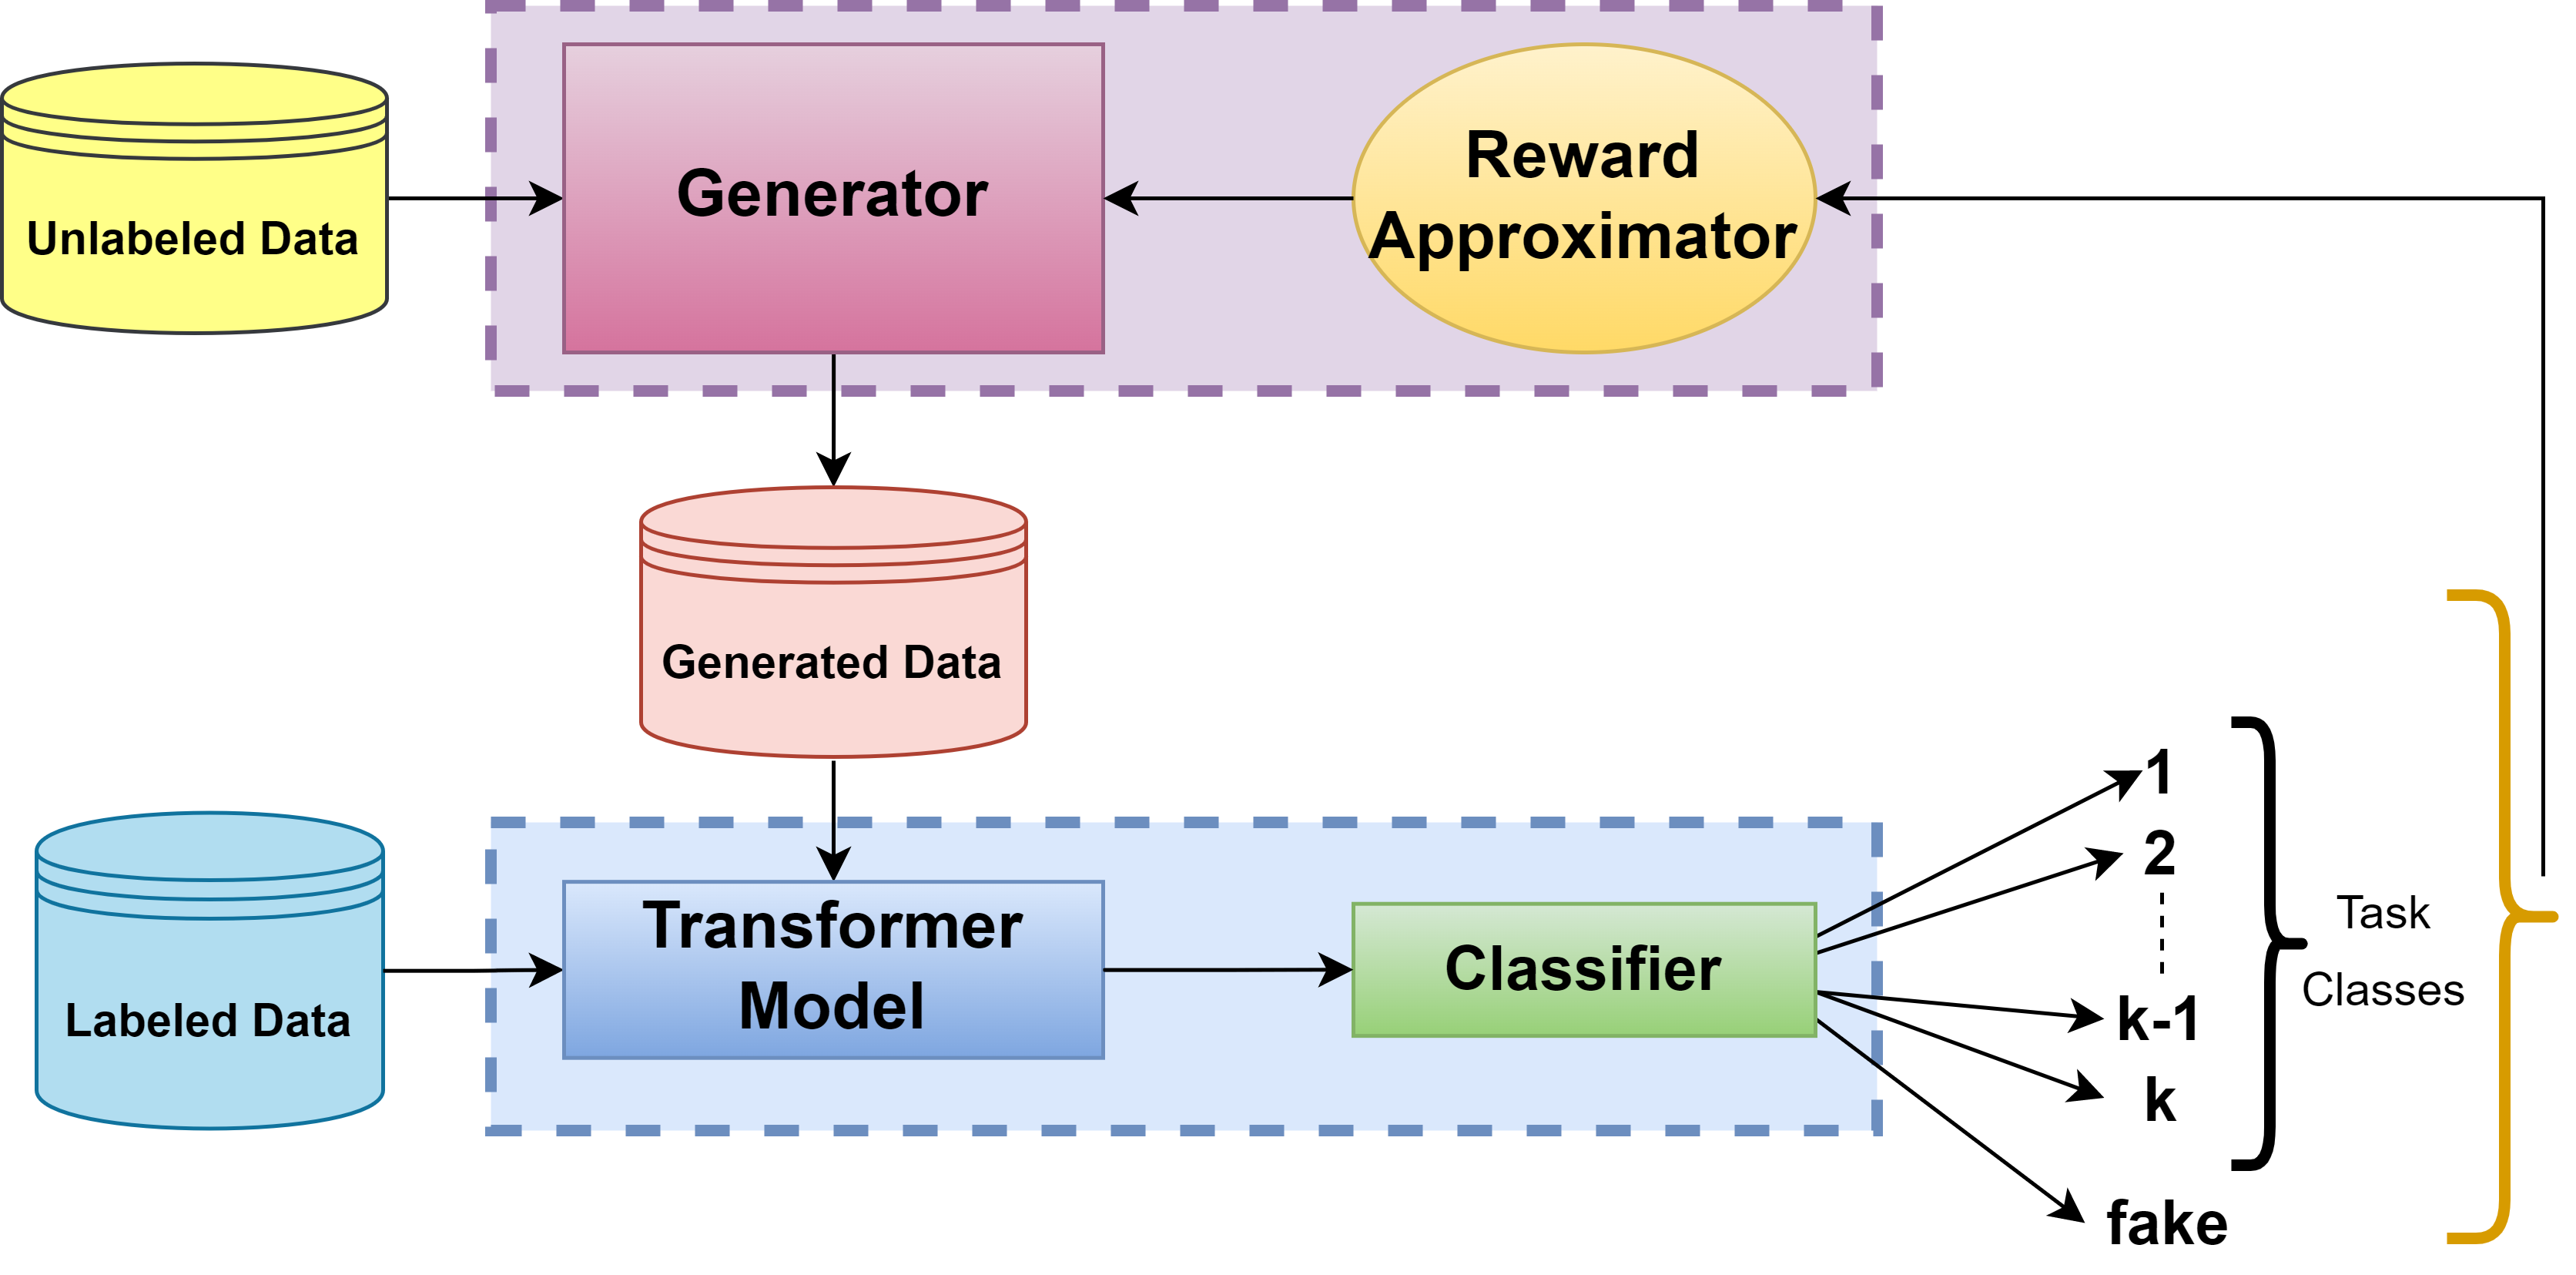
\includegraphics[scale=0.065]{figures/rl-bert.drawio.png}
  \vspace{-1.5em}
  \caption{Architecture of \textit{READ}}
  \label{fig:Plot_RL-BERT_Architecture}
\vspace{-0.5em}
\end{figure}

\textbf{Text Generator $\mathcal{G}$} is implemented by following the IRL, where it trained using the unlabelled dataset $U$ to generate synthetic and diversified texts $U^{\prime}$. Text generation task can be regarded as the generation of the text sequence $x_{1: T}=$ $x_{1}, x_{2}, \cdots, x_{T}$ with a trajectory $\tau = \{s_1, a_1, s_2, a_2, \cdots, s_T, a_T\}$, where $s_t$ is the current state of the previous prediction $x_{1:t}$ and $a_t$ is the action to select the next word $x_{t+1}$. $\mathcal{G}$ is trained to generate real-like examples by maximizing the expected reward $\mathcal{R}(\tau)$.

\textbf{Reward Approximator $\mathcal{R}$} is also defined following IRL as the summation of the rewards of each step with a modification. The reward function at step $t$ is defined using $r_\phi(s_t, a_t)$, where $r_\phi$ is a feed-forward neural network. To bridge the generation and classification processes, we use the  probability $p_{k+1}$ of being classified as fake by the classifier $\mathcal{C}$ as the additional input in the reward function $r_{\phi}\left(s_{t}, a_{t}, p_{k+1}\right)$. The overall reward for a trajectory $\tau$ can be defined as follows:
\begin{equation*} \label{eq:rewardapprox}
R_{\phi}(\tau)=\sum_{t} r_{\phi}\left(s_{t}, a_{t}, p_{k+1}\right)
\end{equation*}

% The reward is calculated using the Reward Approximator $\mathcal{R}$Assuming the real text distribution is $p_{\phi}(\tau)$. The 

% Following the maximum entropy framework by \cite{ziebart2008maximum}, we assume that the texts in training set $U$ are sampled from the distribution $p_{\phi}(\tau)$.


% The text generation process primarily consists of two modules, which are trained alternatively in adversarial setting; (1) Generator $G_\theta$, generates synthetic sample $U^{\prime}$ and (2) Reward Approximator $R_\phi$ that gives reward to generated samples. Our text generation process is motivated by \citet{shi2018toward} work. However, our reward calculation process is different from them. 

% \hspace{-1em}\textbf{Reward Approximator}:
% Following the maximum entropy framework by \cite{ziebart2008maximum}, we assume that the texts in training set $U$ are sampled from the distribution $p_{\phi}(\tau)$.

% \begin{equation}
% p_{\phi}(\tau)=\frac{1}{Z} \exp \left(R_{\phi}(\tau)\right)
% \end{equation}

% \begin{equation}
%   Z=\int_{\tau} \exp \left(R_{\phi}(\tau)\right) d \tau
% \end{equation} 
% Here, $R_{\phi}(\tau)$ an unknown reward function and $Z$ is the partition function.

% Text generator module use unlabelled text $U$ as input, and generates synthetic sample $U^{\prime}$ using \textit{Generator} $G$  (refer {Section \protect\ref{sec:gen}}). Subsequently, sample set $Q$, which is a union of $U$ and $U^{\prime}$ is passed to a Language Model $L_{m}$ for encoding and then \textit{Discriminator} $D$ which acts as a classifier (refer {Section \protect\ref{sec:descriminator}}) provides classification probability $p$ for a text $x \in Q$. During text generation at each step $t$ using classification probability $p$ we calculate the reward using $r_{\phi}\left(s_{t}, a_{t}, p\right)$, where $s_{t}$ and $a_{t}$ denotes the current state and action. The overall reward of trajectory $R_{\phi}(\tau)$ is computed by summing the the rewards of each steps as follows:

% \begin{equation} \label{eq:rewardapprox}
% R_{\phi}(\tau)=\sum_{t} r_{\phi}\left(s_{t}, a_{t}, p\right)
% \end{equation}

% We model $r_{\phi}\left(s_{t}, a_{t},p\right)$ as a simple feed-forward neural network. 

$\mathcal{R}$ is trained to maximize the log-likelihood of the samples in the $U$, whereas $\mathcal{G}$ is trained to maximize the expected reward with an entropy regularization term. We follow IRL framework for defining the training objectives of $\mathcal{R}$ and $\mathcal{G}$, and refer the readers to their work for additional details.

% hence we omit  details and simply use the approximated derv Following IRL, we define the objective as:
% \begin{equation} \label{eq:rewApprx}
%  \mathcal{J}_{r}(\phi) = \mathbb{E}_{\tau \sim p_{\text{}}}  R_{\phi}(x)-\mathbb{E}_{x \sim q_\text{generated}}  R_{\phi}(x)
% \end{equation}

% During the reward computation process, we separately compute reward $\mathbb{E}_{x \sim p_\text{real}} R_{\phi}(x)$ of the real texts $U$ and the reward $\mathbb{E}_{x \sim q_\text{generated}}  R_{\phi}(x)$ for generated synthetic texts $U^{\prime}$. The reward approximator uses both the computed rewards and try to maximize the log-likehood of the samples in the training set $U$:

% \beg in{equation} \label{eq:rewApprx}
%  \mathcal{J}_{r}(\phi) = \mathbb{E}_{x \sim p_{\text{real}}}  R_{\phi}(x)-\mathbb{E}_{x \sim q_\text{generated}}  R_{\phi}(x)
% \end{equation}

% In the above Equation, reward-approximator aims to increase the rewards of the real texts and decrease rewards on generated texts.

% \hspace{-1em}\textbf{Generator}:
% In our proposed network the working of \textit{Generator} is similar to \citet{shi2018toward} work. The \textit{Generator}, generates the synthetic texts $U^{\prime}$ using generator policy $G_\theta$. The objective of the generator policy $G_\theta$ is to maximize the expected reward and to reduce the mis-classification errors from \textit{Discriminator} $D$.

% \begin{equation}
%  \mathcal{J}_{g}(\theta) = \mathbb{E}_{x \sim q_{generated}}\left[R_{\phi}(x)\right] + H\left(q_{generated}(x)\right)
% \end{equation}

% \begin{equation}
% H\left(q_{generated}(\tau)\right)=-\mathbb{E}_{q_{generated}(\tau)}\left[\log q_{generated}(\tau)\right]
% \end{equation}

% Here, $H$ is an entropy term, which can prevent premature entropy collapse and encourage the generator policy $G_\theta$ to generate more diverse texts. 

\textbf{Transformer Model  $\mathcal{M}$} is a pre-trained transformer model to encode any input text to a $d$-dimensional feature representation $h \in \mathbb{R}^d$. \textbf{Classifier $\mathcal{C}$} is defined by following GAN-BERT, where $\mathcal{C}$ is trained to classify any feature representation $h$ in one of the $k$ task categories or into the ${k+1}^{th}$ \textit{fake} category, if the $h$ corresponds to a fake example. 

\textbf{Training objective of $\mathcal{M}$ and $\mathcal{C}$} is defined by minimizing following three losses:  $\mathcal{L}_{l}$ loss on classifying the samples from the labeled dataset $L$ into one of the $k$ classes,  $\mathcal{L}_{r}$ loss for not classifying the samples from $L$ and $U$ as \textit{fake}, and an additional $\mathcal{L}_f$ loss for classifying the generated samples from $U^{\prime}$ as \textit{fake}.
\vspace{-0.5em}
\begin{gather*}
\mathcal{L}_{l} = -\mathbb{E}_{x, y \sim L} \log \left[p(\hat{y}=y \mid x, y \in(1, \ldots, k))\right] \\
\mathcal{L}_{u} = -\mathbb{E}_{x \sim L \cup U} \log \left[1 - p(\hat{y}=y \mid x, y = k +1)\right] \\
\mathcal{L}_{f} = -\mathbb{E}_{x \sim U^{\prime}} \log \left[p(\hat{y}=y \mid x, y = k +1)\right]
\end{gather*}
 where $p$ is the probability vector returned by $\mathcal{C}$ for the input $x$.

\begin{figure*}[!ht]
     \centering
     \begin{subfigure}[b]{0.32\textwidth}
         \centering
         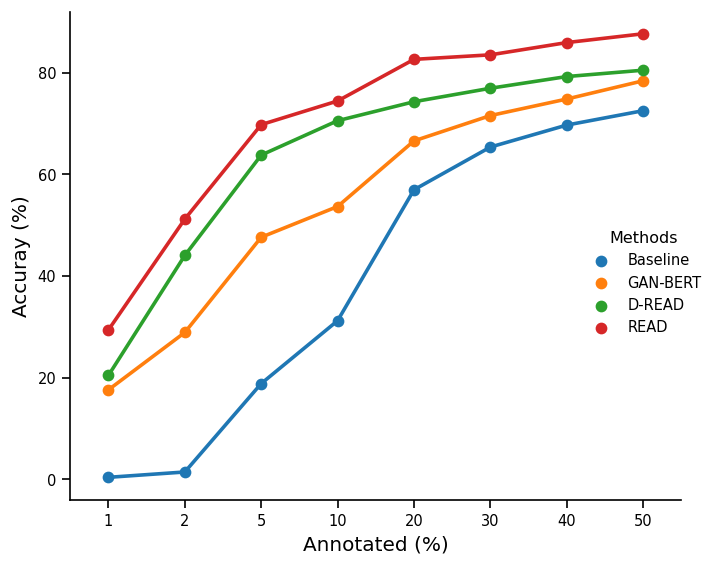
\includegraphics[width=\textwidth]{figures/trec_cf_bert.png}
         \caption{TREC-CF}
         \label{fig:trec_cf_bert}
     \end{subfigure}
     \hfill
     \begin{subfigure}[b]{0.32\textwidth}
         \centering
         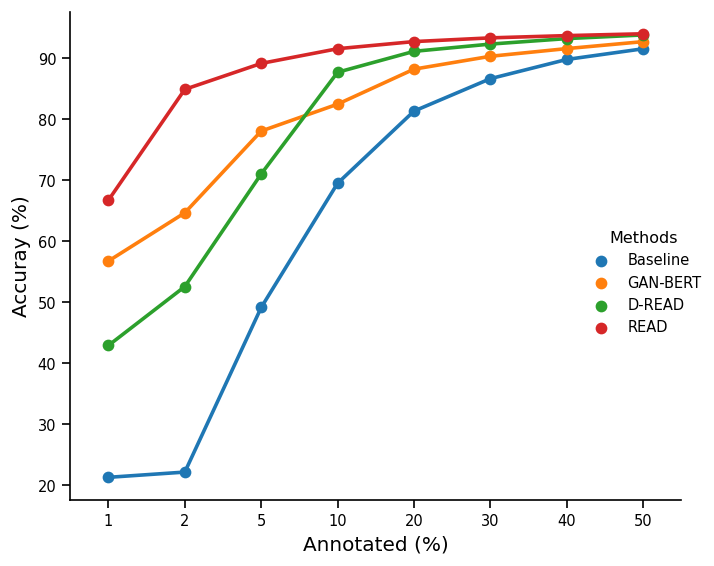
\includegraphics[width=\textwidth]{figures/trec_cc_bert.png}
         \caption{TREC-CC}
         \label{fig:trec_cc_bert}
     \end{subfigure}
     \hfill
     \begin{subfigure}[b]{0.32\textwidth}
         \centering
         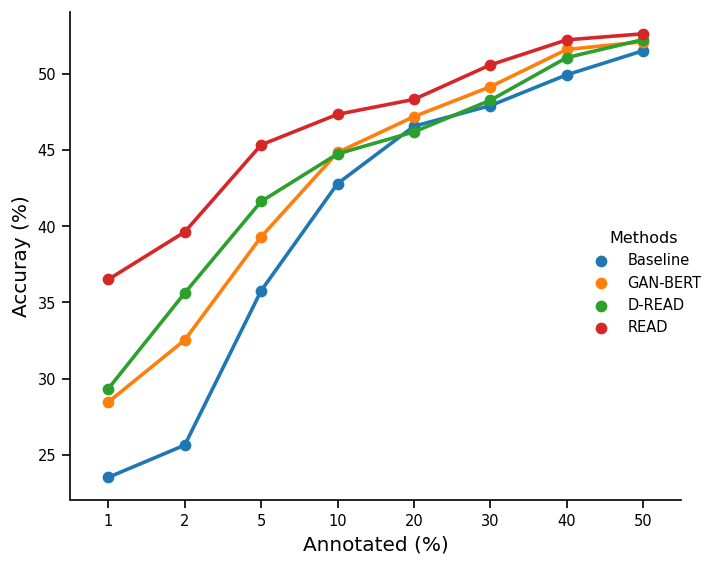
\includegraphics[width=\textwidth]{figures/sst5_bert.png}
         \caption{SST-5}
         \label{fig:sst5_bert}
     \end{subfigure}
     \vspace{-0.5em}
      \caption{Accuracy comparison using BERT model.}
        \label{fig:bert_results}
\end{figure*}

In IRL, the reward function is defined using only current and previous states, whereas in \textit{READ}, the reward function also takes the probability of being fake $p_{k+1}$. As, we are training  $\mathcal{M}$ and $\mathcal{C}$ for identifying the generated samples as the fake class, the probability $p_{k+1}$ of being fake will be high for generated examples whereas it will be low for real text samples. Due to this property, reward function in \textit{\textbf{READ}} will encapsulate the classifier's knowledge along with the real text distribution. Simultaneously, we are training the text generator $G$ to maximize the expected reward using adversarial learning to encourage the generation of samples that are not only  similar in form of states but also having low probability of being identified as fake by $\mathcal{C}$ by fooling the classifier. We hypothesize that this form of adversarial learning based on reinforcement-based text generation instead of feature representation will be more robust towards improving the classifier's generalization capability.

% During the forward pass, samples generated from $G$ are passed to the discriminator $D_\lambda$. The discriminator classify such samples in the fake class with the probability $p$. The generator $G$ use these probability score along with other information to model the reward function. Integrating the probability $p$ in the reward function $R_{\phi}(\tau)$ helps $G_\theta$ to generate synthetic samples which are similar and diverse to the real samples. Such synthetic samples has ability to fool the discriminator by maximizing the classification loss, which helps in improving the performance of multi-class classification. We train the generator via policy gradient, to avoid the differentiation difficulty for discrete data.

% \hspace{-1em}\textbf{Text Classifier}:
% In the proposed network, the \textit{Discriminator} $D$ acts as a classifier. The classifier takes labelled dataset $L$, unlabelled dataset $U$ and generated dataset $U^{\prime}$ as inputs. The samples of these three datasets are passed though a Language Model $L_{m}$ (e.g. BERT, XLMR etc.) to obtain the encoded d-dimensional representation $h_{*} \in \mathbb{R}^{d}$. Here, $h_{*}$ can be either $h_{fake}$ produced by generator or $h_{real}$ for the sample taken from labelled or unlabelled datasets. The encoded representation $h_{*}$ is passed to a Softmax-activated layer, whose output is a $k$ + 1 vector of logits. During training process, when instances are taken from real samples $h_{real}$, \textit{Discriminator} $D$ should classify them in one of the $k$ categories; when instances are taken from generated samples $h_{fake}$ it should classify each example in the $k$ + 1 category. The loss function of $\mathcal{D}$ is defined as: 

% \begin{equation}
% \mathcal{J}_{\mathcal{D}}(\lambda)= \mathcal{J}_{\mathcal{D}_{\text {labelled }}}(\lambda)+ \mathcal{J}_{\mathcal{D}_{\text {unlabelled}}}(\lambda)
% \end{equation}

% \begin{equation}
% \mathcal{J}_{\mathcal{D}_{\text {labelled }}} = -\mathbb{E}_{x, y \sim p_{real}} \log \left[D_\lambda(\hat{y}=y \mid x, y \in(1, \ldots, k))\right]
% \end{equation}

% \begin{equation}
% \mathcal{J}_{\mathcal{D}_{\text {unlabelled}}} = -\mathbb{E}_{x \sim p_{real}} \log \left[1-D_\lambda(\hat{y}=y \mid x, y=k+1)\right]
% \end{equation}

% The $RL$-$LM$ optimize the two competing loss $\mathcal{J}_{\mathcal{D}}(\lambda)$ and $\mathcal{J}_{g}(\theta)$.During back-propagation, the unlabeled examples contribute only to $\mathcal{J}_{\mathcal{D}_{\text {unlabelled}}}$. In the loss computation, the unlabelled loss is only considered if they are erroneously classified into the $k$+ 1 category. In all other cases, their contribution to the loss is masked out. 

% The labeled examples thus contribute to the supervised loss $\mathcal{J}_{\mathcal{D}_{\text {labelled }}}
% $. Finally, the examples generated by $G$ contribute to both discriminator and generator loss. In the training process, the weights of the Language Model $L_{m}$ are updated in order to fine-tune the encoded representation of labelled, unlabelled, and generated data. 

\section{Experimental Details}
\subsection{Dataset}
We have evaluated our method's performance on three sentence classification tasks: Fine Grained Question Classification \textit{\textbf{TREC-QCF}} task \cite{lang1995newsweeder}, Coarse Grained Question Classification \textit{\textbf{TREC-QCC}} task \cite{li2006learning}, and Sentiment Analysis \textbf{\textit{SST-5}} task \cite{socher2013recursive}. We have reported the training and test data statistics in Table \ref{tbl:data} in the Appendix.

% We measure the performance of $RL$-$LM$ by taking different percentage of training samples on the three sentence classification tasks; (i). Fine Grained Question Classification (QC) task using \textit{TREC-QC Fine} (\textbf{TRECF}) dataset, \cite{lang1995newsweeder}, (ii) Question Classification (QC) task on \textit{TREC QC COARSE} (\textbf{TRECC}) dataset \cite{li2006learning} and (iii) Sentiment Analysis (SA) task over \textbf{\textit{SST-5}} dataset \cite{socher2013recursive}. Table \ref{tab:dta} present the details of the datasets.

\subsection{Baselines and \textit{\textbf{READ}}'s Variants}
In our experiments, we compare \textit{READ} with \textbf{GAN-BERT} and \textbf{Baseline} which is a vanilla fine-tuning method without any adversarial training. We experiment with two pre-trained transformer models BERT \cite{devlin-etal-2019-bert} and RoBERTa \cite{liu2019roberta}. To understand the importance of the encapsulation of text generation and adversarial learning, we experiment with disjoint training of text generation and classifier by removing the probability of being fake from the reward function, $r_{\phi}(s_{t}, a_{t})$. We denote the method of disjoint training as \textit{\textbf{D-READ}} in our experiments.

% $RL$-$LM$, we take $BERT$ \cite{devlin-etal-2019-bert} as Language Model, and build $RL$-$BERT$. We measure the performance of $RL$-$BERT$ with the following baselines:

% \begin{itemize}

% \item \textbf{BERT}: Uses $BERT$ \cite{devlin-etal-2019-bert} as encoder and fine-tunes the weight of the same during text classification task using labelled dataset $L$.

% \item \textbf{RoBERTa}: Uses $RoBERTa$ \cite{liu2019roberta} as encoder and fine-tunes the weight of the same during text classification task using labelled dataset $L$.



% \item \textbf{GAN-BERT} \cite{croce2020gan}: extends the fine-tuning of BERT with unlabeled data in a generative adversarial setting. 

% \item \textbf{GAN-RBT}: uses the same architecture as GAN-BERT \cite{croce2020gan} by replacing BERT with $RoBERTa$ as Language Model.



% \item \textbf{RL-BERT}: Use $BERT$ as the Language Model in our proposed architecture of $RL$-$LM$.

% \item \textbf{RL-RBT}: Uses $RoBERTa$ as the Language Model in our proposed architecture of $RL$-$LM$.
% \end{itemize}


\subsection{Training Details}
We followed IRL for implementing text generator and reward approximator. The text generator consists of a LSTM layer with embedding size of 128 and followed by 4 linear layers with dimension of 128 along with a dropout of 0.1. We set the maximum sequence length of the generated sentences to 64. The reward approximator consists of MLPs with 3 hidden layers of 128 dimensions with a dropout of 0.2. The Classifier consists of a hidden layer of 768 dimension followed by $leaky$-$ReLu$ activation function. We have used AdamW \cite{loshchilov2018decoupled} as the optimizer with learning rate of 0.005 for $\mathcal{G}$, 0.004 for $\mathcal{R}$, and 5e-5 for both $\mathcal{M}$ and $\mathcal{C}$. 

\section{Results}
\begin{figure*}
  \centering
  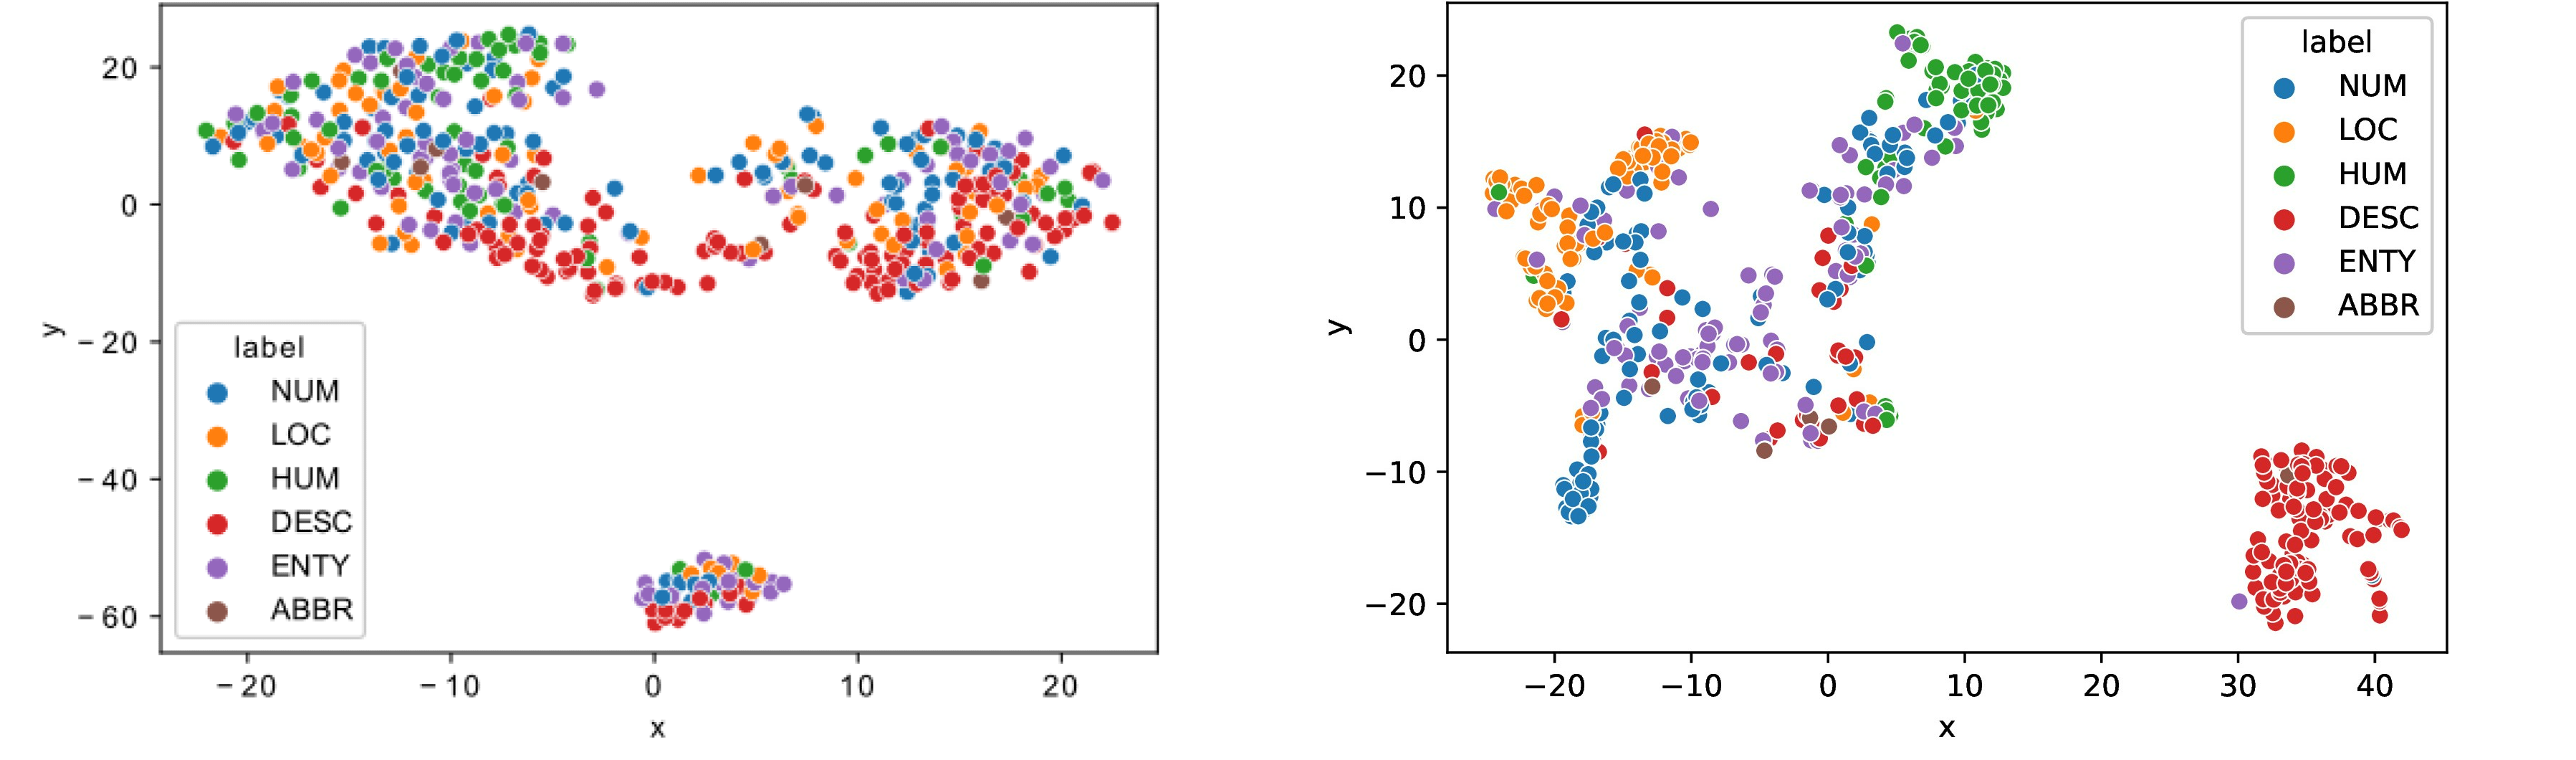
\includegraphics[width=\textwidth]{figures/MergedPlots.png}
%   \vspace{-1.5em}
  \caption{t-SNE Visualization of feature from using Baseline method (left) and  \textit{READ} (right) on TREC-CC task. 
  The class labels are different classes of Questions 'ABBR': Abbreviation, 'ENTY': Entity, 'DESC': Description and abstract concept, 'HUM': Human being, 'LOC': Location, 'NUM': Numeric value.
  }
  \label{fig:tsne_bert}
\end{figure*}

We have reported the accuracy for varying amount of labeled data using BERT pre-trained model in Figure \ref{fig:bert_results}. We observe that the accuracy increases with the increase in the amount of annotated data for all the methods. The Baseline method where no adversarial learning is used performs the worst among all the methods. 

On the TREC-CC task, our method \textit{READ} outperforms the GAN-BERT and Baseline method for all the values of labeled data. The gains are much more significant for the lower amount of labeled data, with gains of 68\% and 26\% over Baseline and GAN-BERT, respectively, when 2\% (108 samples) labeled data is used. Similar to GAN-BERT, the gains from our method starts to diminish with the increase in the amount of labeled data.

We observe similar trends on the SST-5 dataset with \textit{READ} outperforming all the methods in each configuration. Similar to TREC-CC task, the gains from \textit{READ} starts to diminish with the increase in the amount of annotated data. When only 1\% labeled data (85 samples) is used, our method provides 9\% and 14\% of gain over GAN-BERT and Baseline, respectively. 

TREC-CC and SST-5 datasets have only six and five classification categories. However, the TREC-CF dataset has 50 categories, making it a more challenging task than the others. The difficulty of the task is also evident from the fact that the Baseline method achieves almost 0\% accuracy when less than 2\% labeled data is used. We observe that the gains are more significant from \textit{READ} on TREC-CF than the other datasets. We also observe that the trend of diminishing gains with the increase in amount of labeled data is not visible on TREC-CF dataset, with \textit{READ} providing consistent gains for all the values of annotated data.

We have provided a similar analysis using RoBERTa in Figure \ref{fig:roberta_results} in the Appendix. We observe almost similar results to that of BERT, with slightly high accuracy in case of all the methods. It shows that irrespective of the choice of pre-trained transformer model, the proposed approach provides similar gains on all the datasets.

In Figure \ref{fig:bert_results}, we have reported the results for \textit{{D-READ}} method where the text generator and classifier are independently trained, whereas \textit{READ} encapsulates all the components through the reward function. We observe that \textit{D-READ} provides better performance than the GAN-BERT on TREC-CF dataset, showcasing the importance of text generation instead of feature generation. However, it fails to outperform \textit{READ} for all training configurations, demonstrating the importance of encapsulation of all the components.

% The text Generator takes the current state as the input and then predicts the next word using a Policy  G$_\theta$. The Text Generator (G) is implemented as an LSTM \cite{shi2018toward} with embedding dimension of 128 and has 4 hidden layer of 128 dimensions with dropout of 0.1. The maximum sequence length of generated sentences is 64.  The Reward Approximator is a three layer MLP, which has 3 hidden layers of 128 dimensions with dropout of 0.2. Both Generator and Reward Approximator are trained using Adam optimizer with learning rate of 0.005 and 0.004 respectively. 

% The Classifier is an MLP with 1 hidden layer of 768 dimension that is activated by $leaky$-$ReLu$ function and is followed by a $Softmax$ layer for final prediction.


% \begin{figure*}
%      \centering
%      \begin{subfigure}[b]{0.49\textwidth}
%          \centering
%          \includegraphics[width=\textwidth]{figures/TREC QC CoarseBERT.png}
%          \caption{TRECC Dataset with BERT.}
%          \label{fig:QCCoarseBERT}
%      \end{subfigure}
%      \hfill
%      \begin{subfigure}[b]{0.49\textwidth}
%          \centering
%          \includegraphics[width=\textwidth]{figures/TREC QC Coarse-RoBERTa.png}
%          \caption{TRECC Dataset with RoBERTa}
%          \label{fig:QCCoarseRoBERTa}
%      \end{subfigure}
%       \caption{Performance comparison of Models on TRECC  Datasets.}
%         \label{fig:QCCoarse}
% \end{figure*}

% % %%%%%%%%%%
% \begin{figure*}
%      \centering
%      \begin{subfigure}[b]{0.49\textwidth}
%          \centering
%          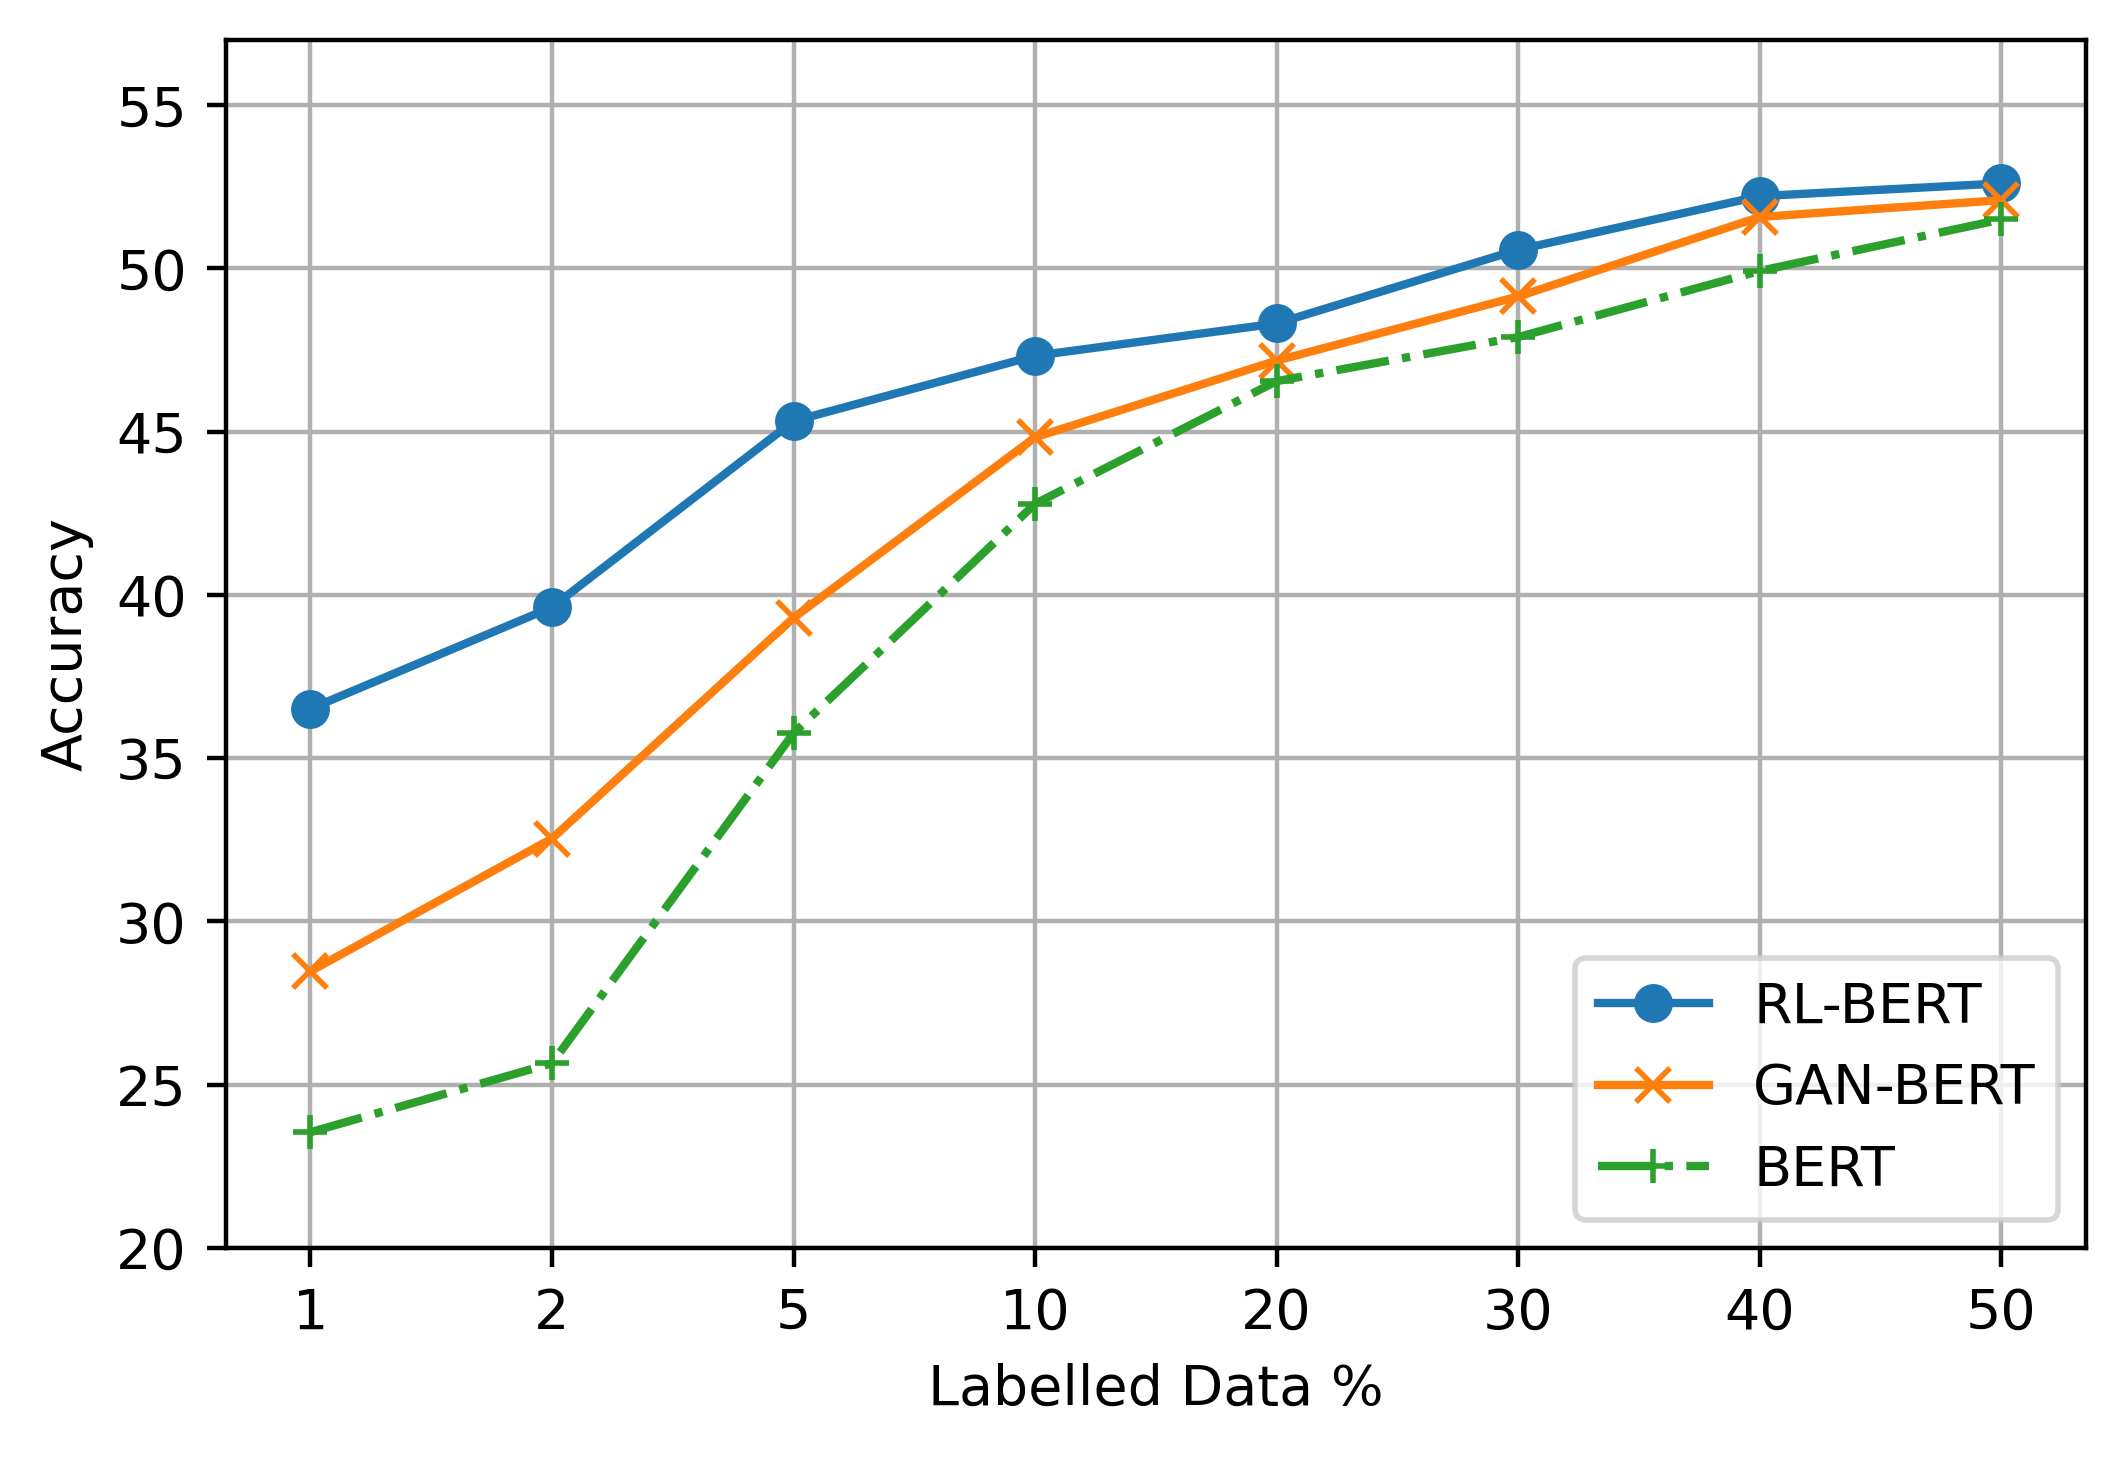
\includegraphics[width=\textwidth]{figures/SST5BERT.png}
%          \caption{SST5 Dataset with BERT.}
%          \label{fig:sst5BERT}
%      \end{subfigure}
%      \hfill
%      \begin{subfigure}[b]{0.49\textwidth}
%          \centering
%          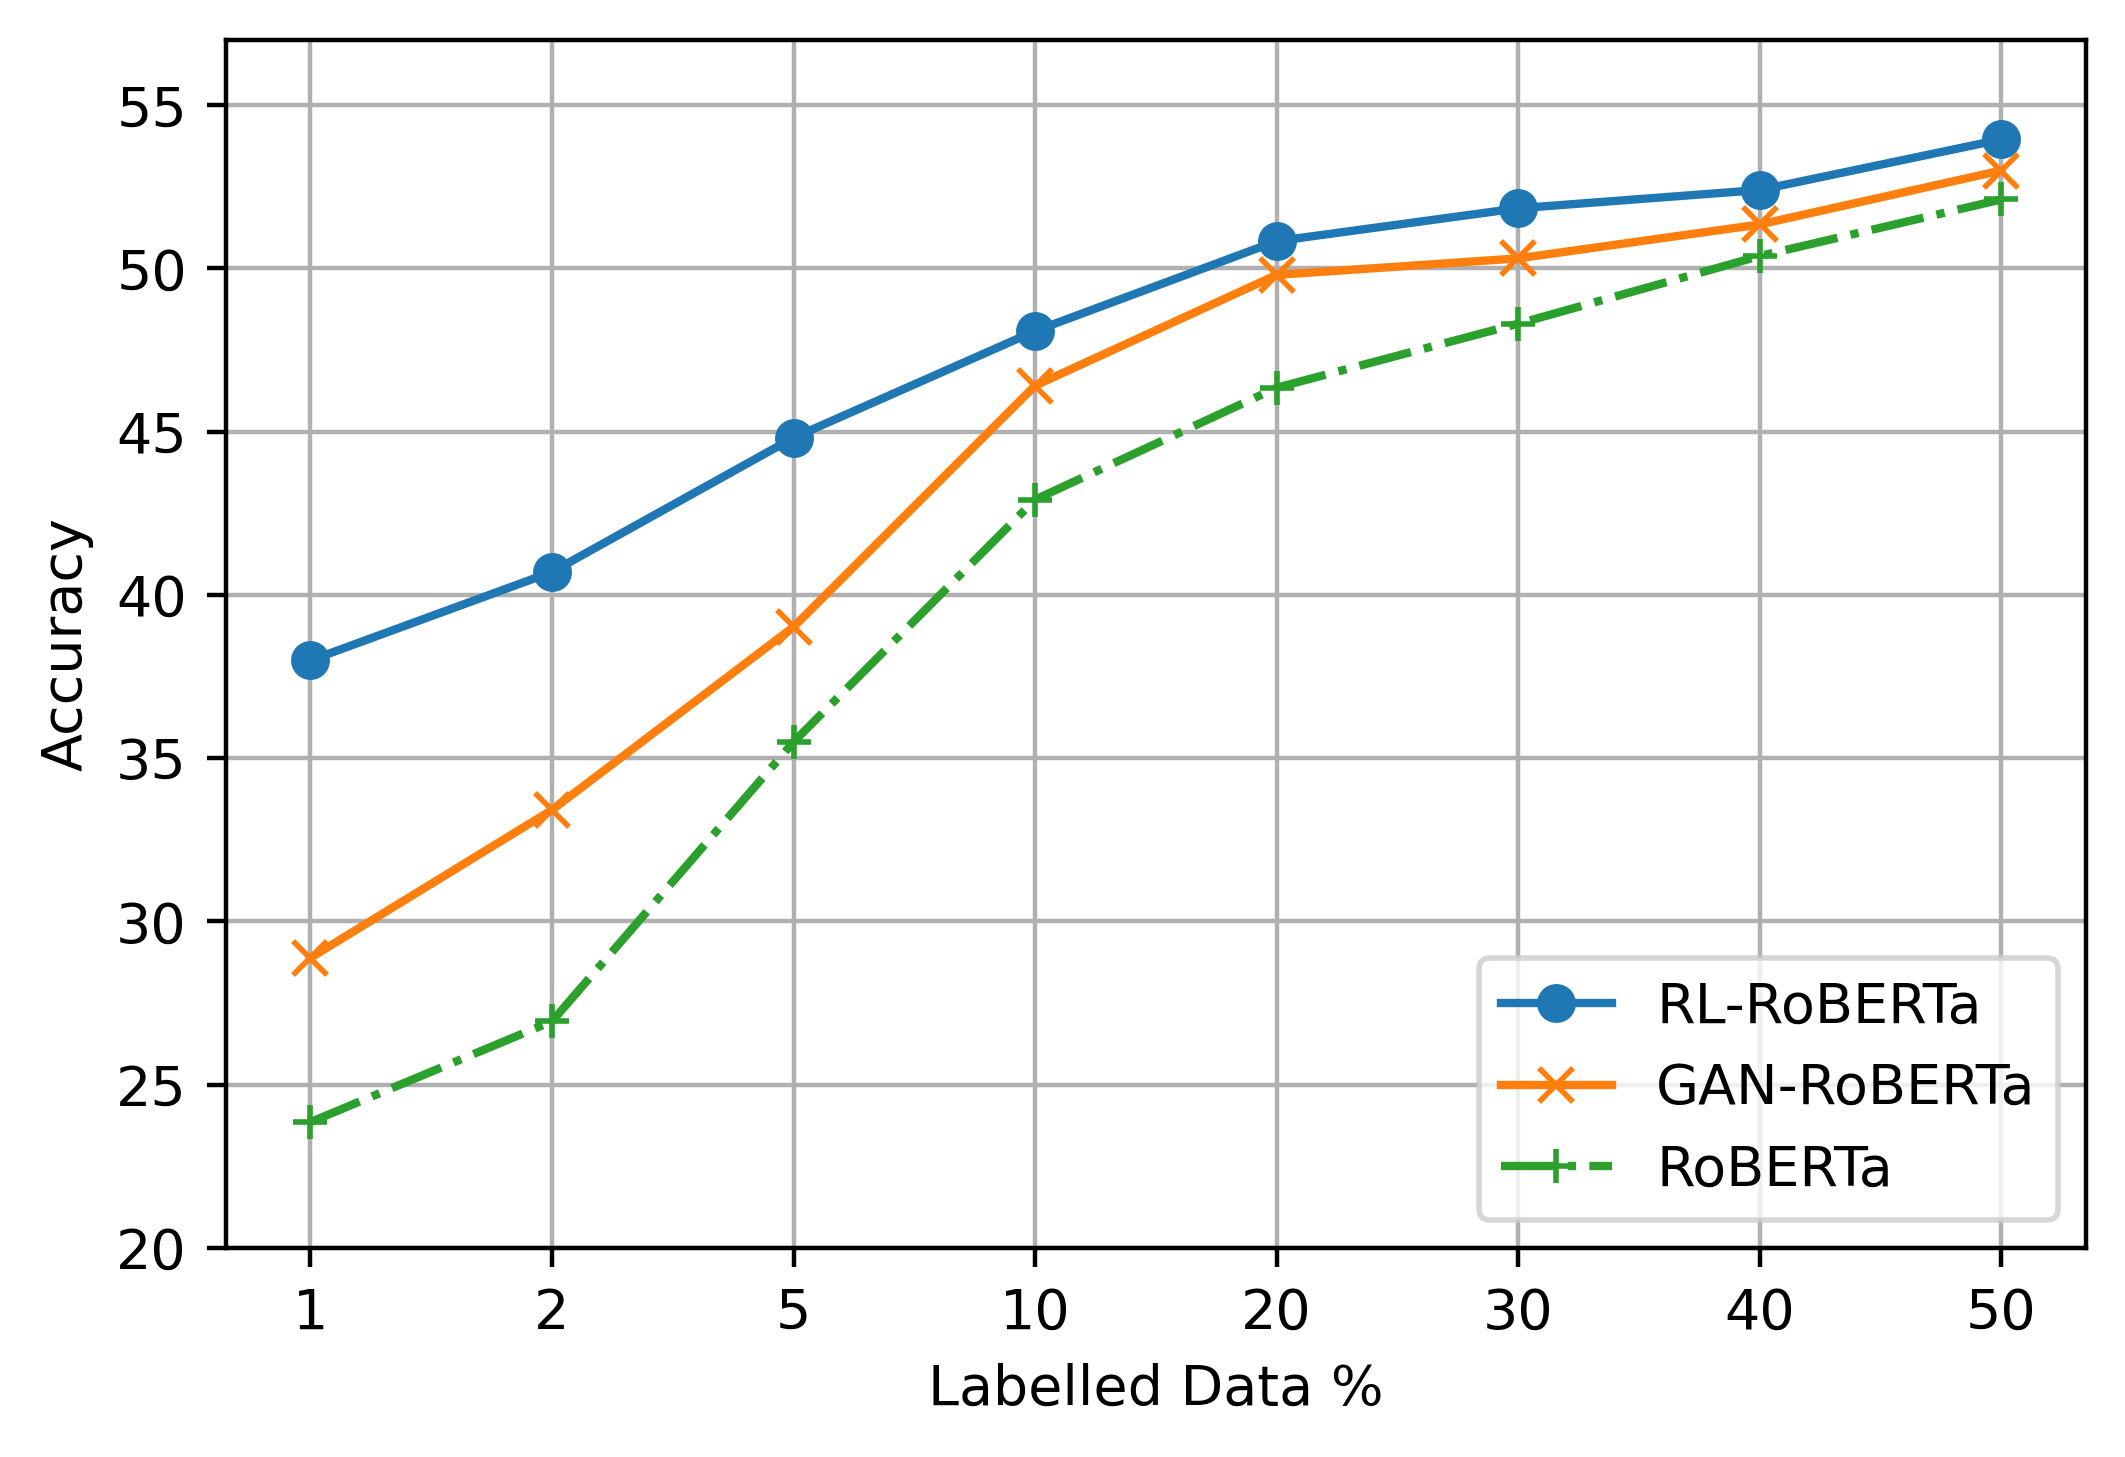
\includegraphics[width=\textwidth]{figures/SST5-RoBERTa.png}
%          \caption{SST5 Dataset with RoBERTa}
%          \label{fig:sst5RoBERTa}
%      \end{subfigure}
%       \caption{Performance comparison of Models on SST5  Datasets.}
%         \label{fig:sst5}
% \end{figure*}

% \begin{figure*}
%         \centering
%      \begin{subfigure}[b]{0.49\textwidth}
%          \centering
%          \includegraphics[width=\textwidth]{figures/TREC QC FineBERT.png}
%          \caption{TREC QC Fine Dataset with BERT.}
%          \label{fig:QCFineBERT}
%      \end{subfigure}
%      \hfill
%      \begin{subfigure}[b]{0.49\textwidth}
%          \centering
%          \includegraphics[width=\textwidth]{figures/TREC QC Fine-RoBERTa.png}
%          \caption{TREC QC Fine Dataset with RoBERTa}
%          \label{fig:QCFineRoBERTa}
%      \end{subfigure}
%       \caption{Performance comparison of Models on TREC QC Fine  Datasets.}
%         \label{fig:QCFine}
% \end{figure*}


% We train all the baseline along with our proposed model ($RL$-$BERT$ and $RL$-$RoBERTa$) by taking different percentage of samples from training datasets. 
% Figure \ref{fig:QCCoarseBERT} shows on \textit{TRECC} dataset, with 2\% of labelled data (108 samples) $RL$-$BERT$ gives 68\% and 26\% better accuracy than $BERT$ and $GAN$-$BERT$, respectively. As we start increasing the percentage of labelled samples during training $RL$-$BERT$ performance start becoming similar to $GAN$-$BERT$ and $BERT$.

% Figure \ref{fig:sst5BERT} shows 
% on \textit{SST-5} dataset with 1\% labelled dataset (85 samples) $GAN$-$BERT$ gives 5\% accuracy gain over $BERT$. Interestingly, $RL$-$BERT$ outperforms $GAN$-$BERT$ with even bigger margin of 9\% on the similar settings. $RL$-$BERT$ continue to outperform $BERT$ and $GAN$-$BERT$ with higher percentage of labelled samples. However, the margin of performance gain starts to minimize with more than 10\% labelled samples.

% The \textit{SST-5} and \textit{TRECC } datasets have five and six classification categories, respectively. However, the \textit{TREC QC FINE} dataset has 50 
% classification labels. Usually 
% with a large number labels, classification task becomes
% more challenging. Figure \ref{fig:QCFineBERT} shows that on 
% \textit{TRECF} dataset until 50\% labelled samples
% $RL$-$BERT$ constantly outperforms $GAN$-$BERT$ and $BERT$ with a bigger margin. It shows that architecture
% of $RL$-$BERT$ helps to improve the performance of classification
% task when number of classification labels are large in number.

% We also evaluate the impact of $RL$-$LM$ by using $RoBERTa$
% as Language Model. 
% Figure \ref{fig:QCCoarseRoBERTa}, \ref{fig:sst5RoBERTa}
% and \ref{fig:QCFineRoBERTa} show that $RL$-$RoBERTa$
% outperforms competing $GAN$-$RoBERTa$ and $RoBERTa$ on  
% \textit{TRECC}, \textit{SST-5} and \textit{TRECF} datasets, respectively. The performance gain of 
% $RL$-$RoBERTa$ over its baseline models on the three datasets are in the similar lines of $RL$-$BERT$.

% In the above result analysis, it is interesting to observe that both variants of our proposed model ($RL$-$BERT$ and $RL$-$RoBERTa$)
% perform much better than baseline models when the number of labelled samples are very less. It shows that irrespective of the choice of Language Model ($BERT$ or $RoBERTa$), our proposed model $RL$-$LM$ has potential to outperform its respective baseline models on all three datasets. This performance gain can be attributed to the semi-supervised co-training framework of $RL$-$LM$ where both \textit{Text Generator} and \textit{Text Classifier} interact with each other and improve themselves. Due to this property \textit{Text Generator} can generate sentences like the real-word sentences and enhances the generalization and descriminative capabilities of the \textit{Text Classifier}. 

% \subsection{RL-Augmented-LM}
% In order to understand the importance of co-training framework of $RL$-$LM$, we build, we build \textbf{$RL$-$AG$-$LM$}, which is one of the modified variant $RL$-$LM$. In \textbf{$RL$-$Augmented$-$LM$} the \textit{Text Generator} and \textit{Text Classifier} components are decoupled from each other. In the first step, the synthetic sentences are generated through Text Generator (refer Section \ref{sec:textgen}) using Unlabelled dataset $U$. During text generation process the reward of trajectory function uses modified version of Equation \ref{eq:rewardapprox}, which is only dependent on $s_{t}$ and $a_{t}$. After generating the synthetic text, in the second step the \textit{Text Discriminator} (refer Section \ref{sec:textdis}) is trained using a Language Model over $k$+1 classes.

% We choose $BERT$ as Language Model to build \textit{$RL$-$BERT$} and 
% \textit{$RL$-$Augmented$-$BERT$}. Subsequently, compare the performance of both the models on different datasets. Figure \ref{fig:augperf} exhibits that \textit{$RL$-$BERT$} outperform 
% \textit{$RL$-$Augmented$-$BERT$} on \textit{SST-5}, \textit{TRECC} dataset when less than 10\% labelled samples are used. The \textit{TRECF}, contains a large number of classification categories. The \textit{$RL$-$BERT$} achieves a constant gain of around 5\% in accuracy over \textit{$RL$-$Augmented$-$BERT$} until 8\% of labelled dataset. However, \textit{$RL$-$BERT$} starts outperforming \textit{$RL$-$Augmented$-$BERT$} with even bigger margin once percentage of labelled samples increases during training process. 

% The performance comparison between  \textit{$RL$-$BERT$} and \textit{$RL$-$Augmented$-$BERT$} empirically proves that integrating the the classification probability $p$ in the reward function $R_{\phi}(\tau)$ and building the co-training framework helps $RL$-$LM$ to enhances the its performance.

\subsection{Generation Quality}
We hypothesize that the quality of synthetically generated text plays a big role in improving the performance of the model. To verify this, we have shown some of the generated samples by mapping it to the original text using cosine-similarity in Table \ref{table:generated_data}. The generated samples are almost similar to the real text with lot of variations, showing the diversity in the generation quality.

\subsection { Discriminative Features}
We have shown the t-SNE \cite{van2008visualizing} visualization of the features from the last layer of the BERT model after fine-tuning Baseline and \textit{READ} method on TREC-CC dataset with 1\% of labeled data in Figure \ref{fig:tsne_bert}. We can see that the features learnt from Baseline are not class-discriminative and are overlapping for lot of classes, whereas the features learnt using \textit{READ} are class-discriminative, with each cluster denoting a class-label. Our method is able to learn class-clusters with just 1\% of labeled dataset, validating the observed gains in the previous sections.

% In order to understand the quality of learnt discriminative features of $RL$-$LM$,
% we take 1\% labelled data from \textit{UIUC} Dataset 
% and train $RL$-$BERT$ and $BERT$. After training we 
% take embeddings of the classification layer of these two models over the test dataset
% and plot the t-SNE graph using the same. Figure \ref{fig:tsne_bert} shows that
% classification embeddings of $RL$-$BERT$ has learnt much better descriminative features compare to $BERT$, which helps $RL$-$BERT$ to perform better in a small labelled data settings.

\section{Conclusion}
In this work, we propose a novel method for improving the generalization capabilities of text classifiers when fine-tuned with limited labeled data. \textit{READ} encapsulate reinforcement-based text generation and classifier through adversarial learning with the help of unlabeled data. We evaluated our method on multiple datasets and observed significant gains over the Baseline and GAN-BERT when very limited data is used. We show the importance of encapsulation through experiments and observed a significant drop in performance with disjoint training. We validated the improvements of \textit{READ} through feature visualization. Our method is only evaluated in English and can be easily extended to other languages. There have been a few works \cite{dong2019unified, li2021pretrained} proposed to improve the text generation quality by utilizing pre-trained transformer models. We plan to extend our approach by integrating these generation methods to improve performance further. 
% Our experiments shows an improvement in the few-shot accuracy of the sentence classification tasks which uses Language Models as Classifier. We evaluated on multiple real world dataset to show that synthetically generating sentences using Adversarial training can help the classifier to increase its robustness and thus the classification accuracy.

% \section{Limitations}
% \begin{itemize}
% % \item the current work is analyzed only only English. We wish to extend this framework for multilingual data.
% \item The performance improvement in GAN-BERT and RL-RoBERTa is due to generation of synthetic sentences which uses unlabeled data. However, acquiring the unlabeled examples in classification tasks like Question answer and sentence pairing is difficult. 
% \item The generated sentences may not be diverse and for every class. This happens sometimes due to mode-collapse in GANs when the generated sentences belong to the same class. 
% \end{itemize}



% In $RL$-$LM$ the quality of synthetically generated text plays a big role
% in improving the performance of the model. In this Section we show that the \textit{Text Generator} (G) generates a synthetic text which is
% human-written like original text. We train $RL$-$BERT$ model on \textit{TRECF} dataset and select some of the synthetically generated text during training process. We map the generated text with the original unlabeled samples using the $cosine$ $similarity$ score. Table \ref{table:generatedExamples1} and Table \ref{table:generatedExamples2} present the samples of original and synthetic text.

% \begin{figure}
%      \centering
    
%       \begin{subfigure}[b]{0.4\textwidth}
%           \centering
%           \includegraphics[width=\textwidth]{figures/TREC QC CoarseAugmented-BERT.png}
%           \caption{TRECC Dataset.}
%           \label{fig:AdultwordCloud}
%       \end{subfigure}
%       \hfill
%       \begin{subfigure}[b]{0.4\textwidth}
%          \centering
%           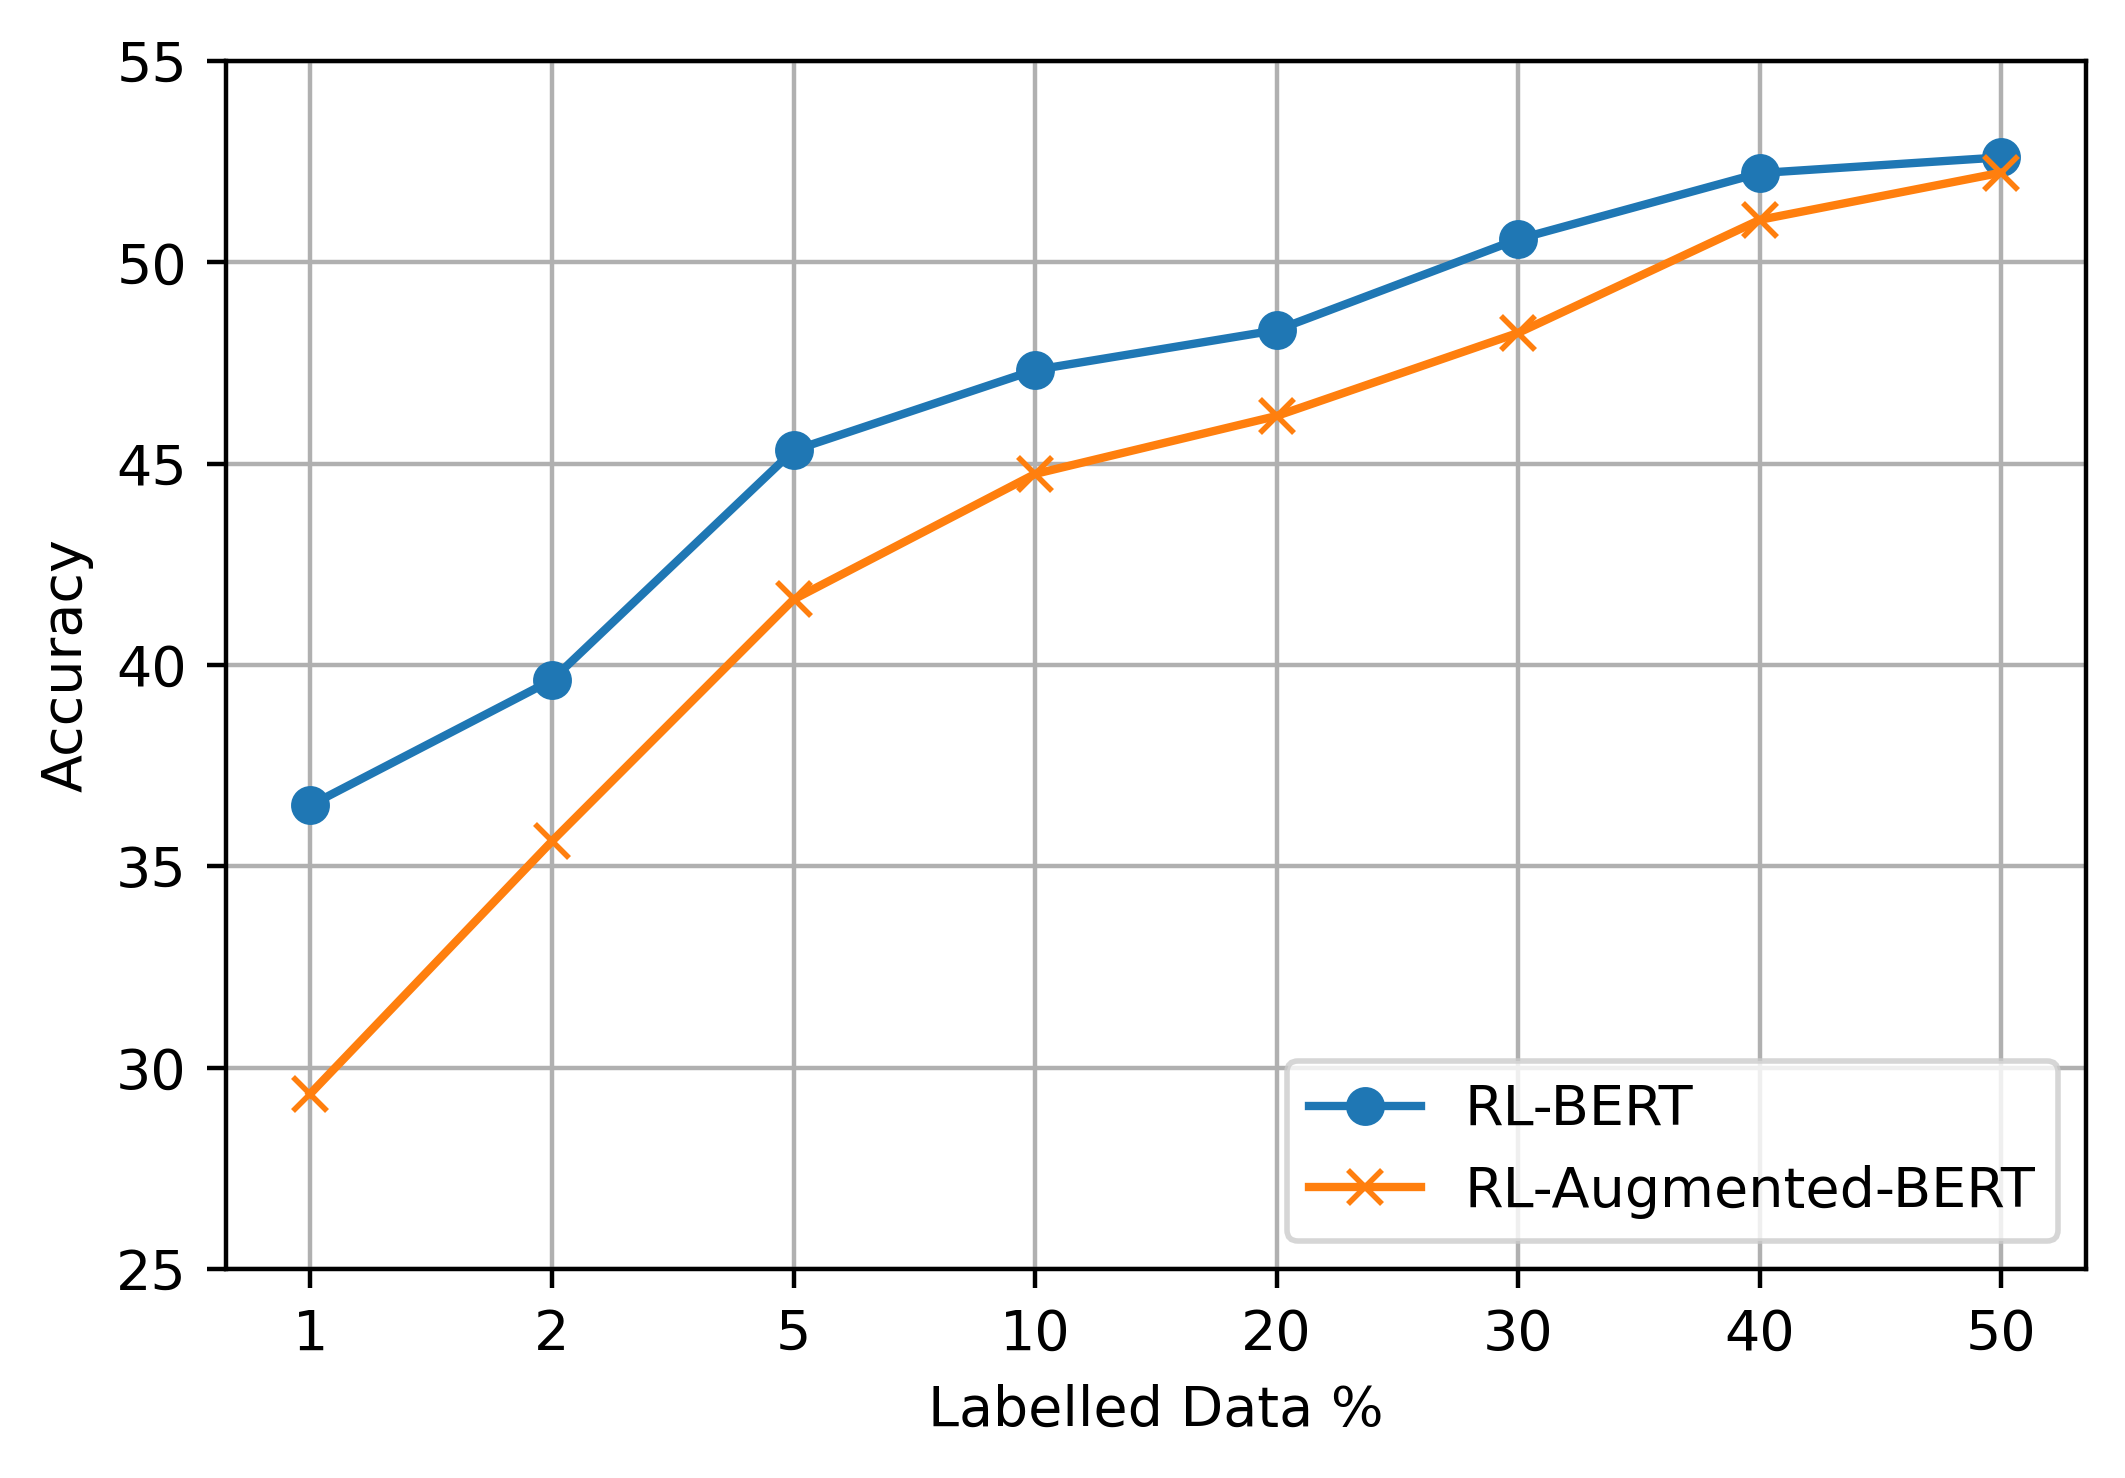
\includegraphics[width=\textwidth]{figures/SST5Augmented-BERT.png}
%           \caption{SST-5 Dataset.}
%           \label{fig:RacywordCloud}
%       \end{subfigure}
%       \hfill
%       \begin{subfigure}[b]{0.4\textwidth}
%           \centering
%          \includegraphics[width=\textwidth]{figures/TREC QC FineAugmented-BERT.png}
%          \caption{TRECF Dataset.}
%           \label{fig:QCFineBERT}
%       \end{subfigure}
%       \caption{Text Classification accuracy of RL-BERT and RL-Augmented-BERT on different Datasets.}
%          \label{fig:augperf}
%  \end{figure}

% \ref{table:generatedExamples1}

% Entries for the entire Anthology, followed by custom entries
\bibliography{anthology,custom}
\bibliographystyle{acl_natbib}

\newpage
\appendix

\section{Data Statistics}
We have provided the statistics of training and test data for each datasets in  \ref{tbl:data}. 

\begin{table}[!]
    \centering
    \small
    \setlength\tabcolsep{2pt}%
    \begin{tabular}{|p{0.3\linewidth} | p{0.2\linewidth} | p{0.15\linewidth} | p{0.15\linewidth}|}
    \hline
        \textbf{Dataset} & \#\textbf{Training Samples} & \#\textbf{Test Samples} & \#\textbf{Labels} \\ \hline\hline
        \textbf{TREC-QCF} & 5452 & 500 & 50 \\ \hline
        \textbf{TREC-QCC}  & 5452 & 500 & 6 \\ \hline
        \textbf{SST5} & 8544 & 2210 & 5 \\ \hline
    \end{tabular}
    \caption{Statistics of datasets.}
\label{tbl:data}
\end{table}

\begin{figure*}[!]
     \centering
     \begin{subfigure}[b]{0.5\textwidth}
         \centering
         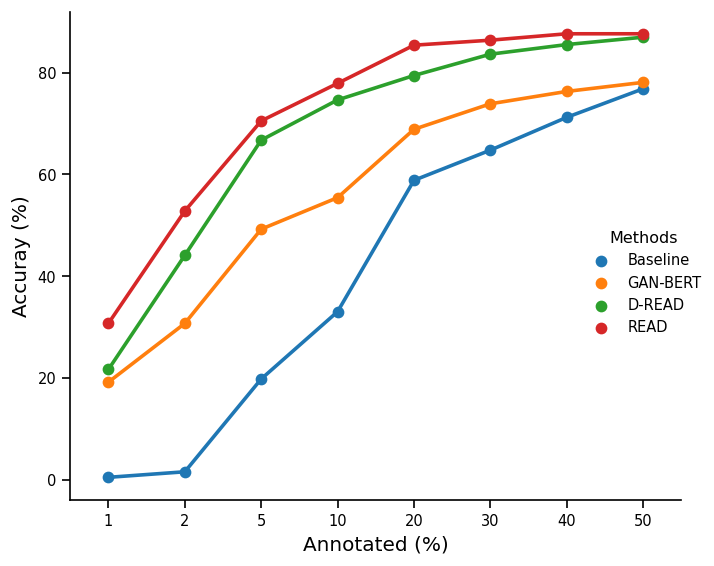
\includegraphics[width=\textwidth]{figures/trec_cf_roberta.png}
         \caption{TREC-CF}
         \label{fig:trec_cf_roberta}
     \end{subfigure}
     \hfill
     \begin{subfigure}[b]{0.5\textwidth}
         \centering
         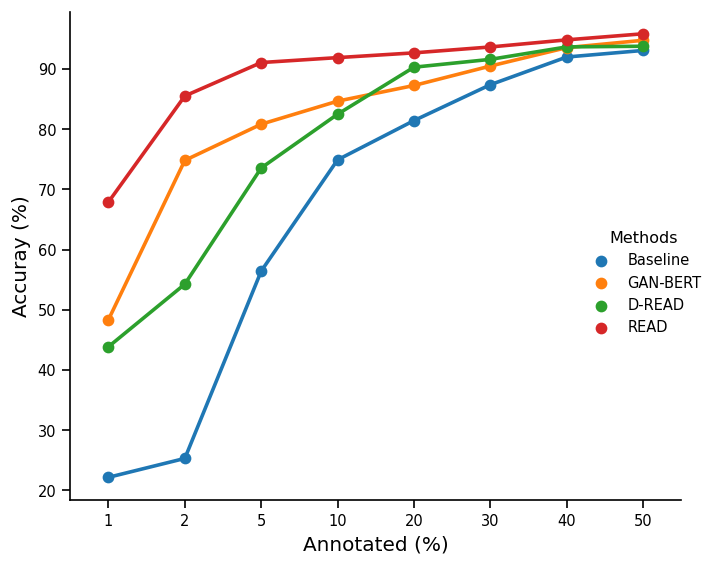
\includegraphics[width=\textwidth]{figures/trec_cc_roberta.png}
         \caption{TREC-CC}
         \label{fig:trec_cc_roberta}
     \end{subfigure}
     \hfill
     \begin{subfigure}[b]{0.5\textwidth}
         \centering
         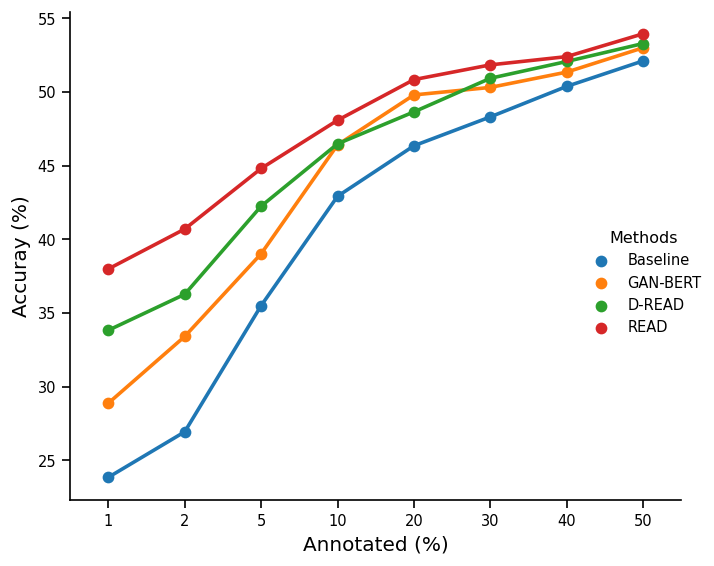
\includegraphics[width=\textwidth]{figures/sst5_roberta.png}
         \caption{SST-5}
         \label{fig:sst5_roberta}
     \end{subfigure}
     \vspace{-0.5em}
      \caption{Accuracy comparison using RoBERTa model.}
        \label{fig:roberta_results}
\end{figure*}

\begin{table*}[!ht]
    \centering
    \begin{tabular}{p{0.5\linewidth}|p{0.5\linewidth}}
    \toprule
    \textbf{Real Text}  & \textbf{Generated Text} \\
    \midrule
How do they find an epicenter?	& How can I find an epicenter?\\
How do they find an epicenter?	& How can I find about an epicenter?\\
How do you find the area of a circle?	& When do you find the area of a circle?\\
How do you find the area of a circle?	& Why do we have to find the area for a circle?\\
How does it make its colors?	& What is an example of a color?\\
How does it make its colors?	& What is a origin of color?\\
How does it make its colors?	& What color were available for?\\
How is the element strontium purified?	& How long is the element strontium purified?\\
How is the element strontium purified?	& What is the element strontium purified?\\
How many Russians have landed on the moon?	& How Russians have landed on the moon?\\
How many Russians have landed on the moon?	& How many astronauts have been on the moon?\\
How many Russians have landed on the moon?	& How many people have been on the moon?\\
How many Russians have landed on the moon?	& How many Americans landed on the moon?\\
Boxing Day is celebrated on what date?	& What was the date of Boxing Day?\\
Boxing Day is celebrated on what date?	& When was Boxing Day?\\
CPR is the abbreviation for what?	& What does CPR stand for?\\
CPR is the abbreviation for what?	& What is the meaning of `` CPR ''?\\
CPR is the abbreviation for what?	& What is the definition of ` CPR ''?\\
\bottomrule
\end{tabular}
\caption{Generated data in TREC-CC Fine dataset}
\label{table:generated_data}
\end{table*}

% \begin{table*}[!ht]
%     \centering
%     \caption{Generated data in TREC QC Fine dataset}
%     \label{table:generatedExamples1}
%     \begin{tabular}{|p{0.5\linewidth}|p{0.5\linewidth}|}
%     \hline
%     \textbf{Real Text}  & \textbf{Generated Text} \\ \hline
%     By how much will the California state gas tax rise by the year 2000 ? & What will the California gas tax be in the year 2000 ? \\ \hline
%         By how much will the California state gas tax rise by the year 2000 ? & What will the California gas tax be in next five years ? \\ \hline
%         What is the name of David Letterman 's dog ? & What 's the name of David Letterman 's dog ? \\ \hline
%         What is the name of David Letterman 's dog ? & What is the name of David Letterman 's dog ? \\ \hline
%         What is the name of David Letterman 's dog ? & What was the name of David Letterman 's dog ? \\ \hline
%         What is the name of David Letterman 's dog ? & What is the name for David Letterman 's dog ? \\ \hline
%         What is the name of David Letterman 's dog ? & What is the nickname for David Letterman 's dog ? \\ \hline
%         What is the name of David Letterman 's dog ? & What magazine is the name of David Letterman 's dog printed on? \\ \hline
%         When was the first Barbie produced ? & When is the first Barbie produced ? \\ \hline
%         When was the first Barbie produced ? & When was the first Barbie produced ? \\ \hline
%         When was the first Barbie produced ? & What year was the first Barbie produced ? \\ \hline
%         When was the first Barbie produced ? & Who was the first Barbie produced ? \\ \hline
%         What 's the population of Biloxi , Mississippi ? & What is the state nickname of Mississippi ? \\ \hline
%         What 's the population of Biloxi , Mississippi ? & What state has a capital of Mississippi ? \\ \hline
%         What 's the population of Biloxi , Mississippi ? & What is the origin of U.S. state which has nickname of Mississippi ? \\ \hline
%         What war saw a naval battle between the luxury liners Cap Trafalgar and the Carmania ? & What film saw a naval battle between the luxury liners Cap Trafalgar and the Carmania ? \\ \hline
%         What war saw a naval battle between the luxury liners Cap Trafalgar and the Carmania ? & What war saw over between the luxury liners Cap Trafalgar and Carmania ? \\ \hline
%         What war saw a naval battle between the luxury liners Cap Trafalgar and the Carmania ? & What is the name of a famous battle between the luxury liners Cap Trafalgar and the Carmania ? \\ \hline
%         What war saw a naval battle between the luxury liners Cap Trafalgar and the Carmania ? & What was the name of the famous battle between the luxury liners Cap Trafalgar and the Carmania ? \\ \hline
%         What war saw a naval battle between the luxury liners Cap Trafalgar and the Carmania ? & What is the name of the famous battle between the luxury liners Cap Trafalgar and the Carmania ? \\ \hline
%         Mississippi is nicknamed what ? & What is the name of Mississippi 's ? \\ \hline
%         Mississippi is nicknamed what ? & What was the name of Mississippi ? \\ \hline
%         Mississippi is nicknamed what ? & What was the name of Mississippi for ? \\ \hline
%         Mississippi is nicknamed what ? & What is the state nickname of Mississippi ? \\ \hline
%         Mississippi is nicknamed what ? & What 's the name of Mississippi 's called Acquaintance ? \\ \hline
%         Mississippi is nicknamed what ? & What is the origin of U.S. state nickname of Mississippi ? \\ \hline
%         Mississippi is nicknamed what ? & What is main city of Mississippi 's ? \\ \hline
%     \end{tabular}
% \end{table*}

\end{document}
